

\section{$P_N$-Solver}
\label{sec:pnsolver}



Expanding, discretizing and working with the $P_N$-equations gets increasingly complex for higher order and is arduous and error prone if done by hand. We tackle this problem by expressing the RTE in a computer algebra representation and apply the discretization in angular and spatial domain using manipulation passes on the representation.

The discretized $P_N$-equations are then rendered into source code and compiled. We refer to this as the stencil code. It allows fast construction of the linear system $A\vec{u}=\vec{Q}$ for arbitrary resolution and RTE parameters and has no dependency on the computer algebra framework anymore.

Finally, the generated linear system is solved using standard methods. The solution $\vec{u}$ represents the discretized radiance field $\widehat{L}$, which is evaluated using trilinear interpolation of the SH coefficients. An overview of the solver is given in figure~\ref{fig:pnsolver}. Each step will be described in more detail in the following subsections.

\subsection{Computer Algebra Representation}

Our computer algebra representation is based on mathematical expression trees, which are hierarchies of expression instances. Those can be basic primitives, such as numbers, variables or special symbols, such as the Kronecker delta or imaginary number. Other expression types, such as integrals, derivatives, sums, products and functions build the hierarchy by referencing child expressions.

Our framework further provides manipulators, which can be executed on expressions. We implemented all manipulations, which were required for the derivation of the $P_N$-equations. This includes operations, such as application of the distributive law, substitution, constant folding, reordering of nested integrals, application of identities up to more complex operations, such as factorization of unknowns and discretization of spatial variables. The derivation steps of the real-valued $P_N$-equations in the supplemental material were all carried out using our framework.

\begin{figure}[h]
\centering
\begin{subfigure}{0.45\columnwidth}
\missingfigure{test}
\end{subfigure}%
\hspace{0.05\columnwidth}
\begin{subfigure}{0.45\columnwidth}
\missingfigure{test2}
\end{subfigure}%

\begin{subfigure}{0.45\columnwidth}
\missingfigure{test}
\end{subfigure}%
\hspace{0.05\columnwidth}
\begin{subfigure}{0.45\columnwidth}
\missingfigure{test2}
\end{subfigure}%
\vspace{-0.2in}
\icaption{The computer algebra representation is constructed using API commands provided by our framework (top left) and represented internally as an expression tree (top right). Additional API commands (bottem left) allow valid transformations, which modify the expression tree accordingly (bottom right).}
\end{figure}

Finally, frontends allow rendering the expression tree into different forms. We implemented frontends for rendering expression trees to \LaTeX and C++ source code. The equations in the supplemental material were almost all rendered by the former. The latter was used for generating the stencil code used by our solver.

Note that our framework is different from a computer algebra system (CAS), in that our framework only deals with representation and manipulation of expressions, and is not concerned with finding answers to mathematical problems. 

\subsection{Discretization}

The result of the discretization in angular domain are the real-valued $P_N$-equations. We arrived at the consice form in equations~\ref{eq:rpn_m_<_z}-~\ref{eq:rpn_m_>_z} using our framework. However, once the compact form was found, we used it directly as input to our solver.

The discretization code iterates over all $l,m$-pairs up to order $N$ and chooses either equation~\ref{eq:rpn_m_<_z}, equation~\ref{eq:rpn_m_=_z} or equation~\ref{eq:rpn_m_>_z}, according to the sign of $m$. All occurances of $l$ and $m$ are replaced with their actual values.

The spatial discretization is done by parsing the expression tree of each equation from the root. All occurances of the continuous positional variable $\vec{x}$ are replaced by discrete voxel coordinates $i,j,k$, whose values are retrieved from the top of a stack. The stack is kept by the parser and is initialized with the voxel at $(0,0,0)$. We refer to the space of the discretized $P_N$-equations as stencil space.

Whenever the parser encounters a differential operator, the current voxel position is shifted and pushed to the stack. Then the child expression is parsed and multiplied with a weight value, followed by popping the stack. This is done for each element of a central difference stencil, which provides the offset and weight values (referencing the voxelsize variable). The dimension of the stencil is given by the derivation variable of the operator. Nested derivatives are handled naturally and produce higher order finite difference stencils as expected.

Another aspect to consider during discretization is the location of the variables and unknowns. As we will see later, our solver needs to support staggered grids, where the SH coefficients are not all located at the voxel center (collocated). Some also can be located at the faces, edges and intersections of voxels (staggered).

Our solver therefore supports placement of coefficients at arbitrary staggered grid locations. Whenever a coefficient is encountered during expression tree parsing for discretization, the parser checks how its location is related to the current location on the top of the stack. Depending on how the two are located to each other, the parser returns an expression, which interpolates the coefficients at the requested offset from its surrounding locations, or it returns the coefficient itself, if it happens to coincide. This is also done for RTE parameters, such as $\sigma_t$ or $p^{l,m}$, which are always located at the voxel center. The position stack of the parser is initialized with the staggered grid location defined by the coefficient, which is associated with the $l,m$-pair of the equation currently being discretized.

\subsection{Stencil Code Generation and System Building}

After applying the discretization step to the expression tree of the $P_N$-equations, it is used to generate the stencil code. In numerical analysis, a stencil is an arrangement of voxels and weights, that relate values at different locations to each other and form the basis for propagating rows in the system matrix $A$ and RHS vector $\vec{Q}$ with values. The name comes from the fact, that the geometric structure and weights of the configuration do not change, when applied to different voxels. The same is true for the $P_N$-equations and we use this fact to generate a single function, which propagates rows in $A$ and $\vec{Q}$ for a given voxel.

The $P_N$-equations express, how each coefficient of a voxel depends on other coefficients of the same or adjacent voxels. The unknowns in the terms give information about the coefficient index and voxel offset, and therefore identify a column offset in the matrix $A$. The factors to these coefficients may contain evaluations of RTE parameters, such as $\sigma_t$. Therefore, these factors can not be determined during stencil generation, but are rendered into code expressions, which are executed as part of the stencil function during runtime. Because the stencil code has been generated in stencil space relative to the voxel at $(0,0,0)$, we can run the same stencil code for every voxel, by simply applying an offset accordingly. 

The $P_N$-equations have been discretized, and the stencil has been generated, without any notion of domain boundaries and boundary conditions (BC). Our solver supports Neumann BC and Dirichlet BC. They are handled transparently by the code which runs the stencil. Whenever the stencil writes into $A$ for a boundary coefficient, the framework will either ignore the write operation (Dirichlet BC) or write into the row and column in $A$ of the same coefficient at the closest voxel inside the domain (Neumann BC).

In order to respect the boundary correctly, additional coefficients (which contribute additional rows and columns in $A$ and $\vec{Q}$) are necessary at boundary voxels (see Figure~\ref{fig:staggeredgrid}). This requires careful managegment and bookkeeping of coefficient indices, which is done transparently by the code running the stencil.


\begin{figure}[h]
\centering
\begin{subfigure}{0.45\columnwidth}
%\missingfigure{test}
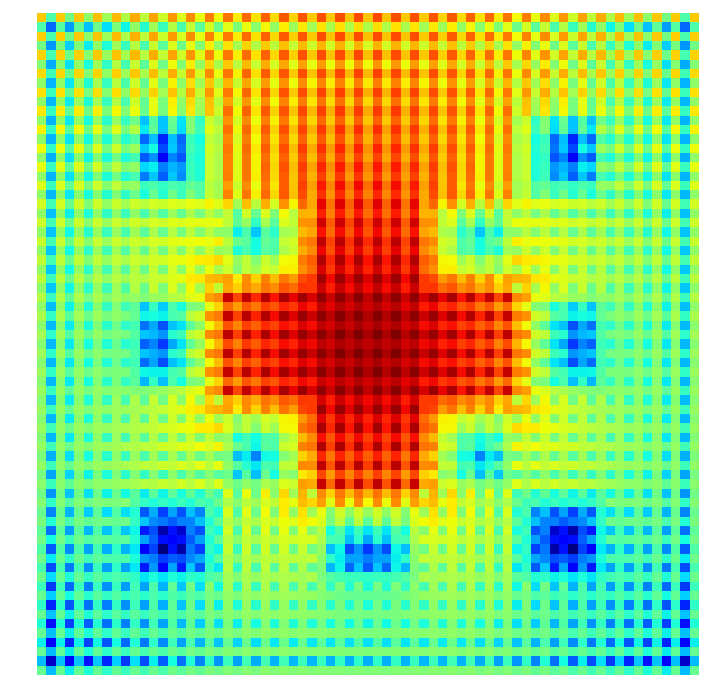
\includegraphics[width=\columnwidth]{images/checkerboard2d_p1_collocated.png}
\end{subfigure}%
\hspace{0.05\columnwidth}
\begin{subfigure}{0.45\columnwidth}
%\missingfigure{test2}
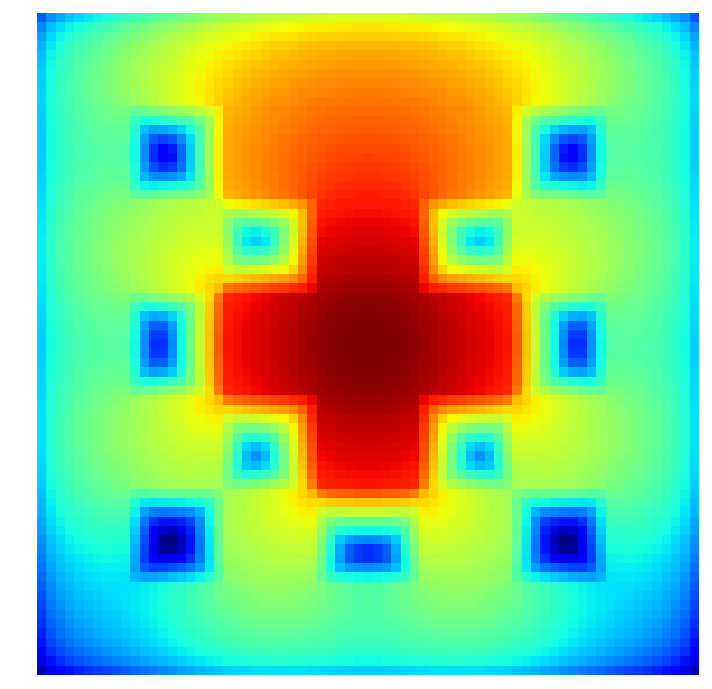
\includegraphics[width=\columnwidth]{images/checkerboard2d_p1_staggered.png}
\end{subfigure}%
\vspace{-0.1in}
\icaption{The solution of our solver for the 2D-checkerboard problem with collocated grids (left), where all coefficients are located at the cell centers. It suffers from severe oscillating artifacts, which are removed by offsetting the coefficient locations using staggered grids (right).}
\label{fig:artifacts}
\end{figure}



\subsection{Solving}

After running the stencil code for every voxel, the system matrix $A$
and RHS vector $\vec{Q}$ are propagated with values and can be used with standard methods for solving systems of linear equations. The number of rows is determined by the number of voxels times the number of coefficients per voxel and can therefore become very large for high resolution and high truncation order. The matrix $A$ is squared and fortunately very sparse, due to finite differences and the structure of the $P_N$-equations. Unfortunately, it also is non-symmetric (due to the transport term) and not diagonal dominant, which rules out many standard methods for solving linear systems. We adress this by solving the normal form $A^TA\vec{u}=A^T\vec{Q}$ instead. This gives a symmetric and positive definit system matrix $A^TA$, albeit with a higher condition number.



\begin{figure}[h]
\centering
\begin{subfigure}{0.45\columnwidth}
\missingfigure{test}
\end{subfigure}%
\hspace{0.05\columnwidth}
\begin{subfigure}{0.45\columnwidth}
\missingfigure{test2}
\end{subfigure}%
\vspace{-0.2in}
\icaption{Staggered grids cause a shifted boundary on the right and upper side of the domain (left). The boundary is correct after introducing additional unknowns (red) at boundary voxels (right).}
\label{fig:staggeredgrid}
\end{figure}


%Matrix $A$ and vector $\vec{Q}$ are constructed after applying the stencil for every voxel.



%\subsection*{CDA vs. $P_1$}
%\begin{itemize}
  %\item CDA is a degenerated form of $P_1$. It is derived by isolating the flux-vector on one side of the vector-equation formed by the $l=1$ SH-band equations. This isolation requires division by the extinction coefficient, introducing a $\frac{1}{\sigma_t}$ factor which diverges as $\sigma_t$ approaches zero. Thresholding to some minimum is required, in order to be able to solve the system for vacuum regions.
  %\item $P_1$ does not require any thresholding of $\sigma_t$ as it does not contain $\sigma_t$ as a denominator. It therefore can deal with vacuum regions without modifications.
  %\item (needs validation) Further, in the presence of vacuum or near vacuum regions, the condition number for CDA is higher than for $P_1$, because of small extinction values in the denominator of the diffusion coefficient.
  %\item Using the normal form for CDA will further increase the condition number when vacuum regions are present and significantly decreases convergence.
%\end{itemize}

